22. $y=|x|+|x+2|=\begin{cases} 2x+2,\ x>0,\\ 2,\ x\in[-2;0],\\ -2x-2,\ x<-2.\end{cases}$
$$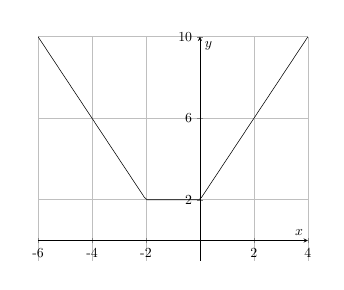
\begin{tikzpicture}[scale=0.5]
\begin{axis}[
    axis lines = middle,
    grid=major,
    legend pos={south west},
    xlabel = {$x$},
    ylabel = {$y$},
    ymin=-1,
    %ymax=250,
    xtick={-6, -4, -2, 2,4},
    xticklabels={-6, -4, -2, 2,4},
    ytick={-2, 6, 2, 10},
    yticklabels={-2, 6, 2, 10}             ]
	\addplot[domain=-6:4, samples=100, color=black] {abs(x)+abs(x+2)};
%\addplot[domain=-3.1:2.5, samples=100, color=red] {70*abs(1-2*abs(abs(x)-2))-10*x^2+10*x-70};
	%\addlegendentry{$\text{Рис. 1}$};
\end{axis}
\end{tikzpicture}$$
